\documentclass[aspectratio=169]{beamer}
%\usetheme{CambridgeUS}
%\usecolortheme{beaver}

%\usefonttheme{serif}
%\usepackage{helvet}

\usefonttheme{serif}     % Font theme: serif
%\usepackage{ccfonts}     % Font family: Concrete Math
\usepackage[T1]{fontenc} % Font encoding: T1

\setbeamersize{text margin left=42pt,text margin right=42pt} 
\setbeamertemplate{navigation symbols}{}
\setbeamertemplate{itemize items}[default]

\beamertemplatenavigationsymbolsempty

\definecolor{fore}{RGB}{51,51,51}
\definecolor{back}{RGB}{255, 254, 250}
\definecolor{title}{RGB}{ 255, 15, 0}
\definecolor{links}{RGB}{18, 168, 255}

\setbeamercolor{titlelike}{fg=title}
\setbeamercolor{normal text}{fg=fore,bg=back}
\setbeamercolor{alerted text}{fg=title}
\setbeamercolor{itemize item}{fg=title}
\setbeamercolor{enumerate item}{fg=title}
\hypersetup{colorlinks,urlcolor=links}

% for code https://kbroman.org/blog/2013/10/07/better-looking-latexbeamer-slides/
\usepackage{listings}
\definecolor{keywords}{RGB}{255,0,90}
\definecolor{comments}{RGB}{60,179,113}
\lstset{language=Python,
keywordstyle=color{keywords},
commentstyle=color{comments}emph}

% fonts
\usepackage[sc]{mathpazo}


% title info
\title{\textbf{Maps / Data / GIS}}
\subtitle{\textbf{GGR424 - Transportation Geography \& Planning}}
\author{Jeff Allen}
\institute{University of Toronto}
\date{February 14, 2022}


\begin{document}
	
\begin{frame}
	\titlepage	
\end{frame}




\begin{frame}
	
	\textbf{Announcements}
	
	\begin{itemize}
		\item In-person class moved to SS2125
		\item Transportation data analysis assignment due March 3
		\item Project proposal due March 10
	\end{itemize}
	
\end{frame}




\begin{frame}
	
	\textbf{Today}
	
	
	\begin{itemize}
		
		\item Travel behaviour data
		\begin{enumerate}
			\item Travel Surveys
			\item Observation/Sensor Data (e.g. GPS)
		\end{enumerate}
		\item Demoing a few things in GIS / chat about the next assignment
		
	\end{itemize}
	
	
\end{frame}




\begin{frame}
	
	\textbf{Travel Behaviour Data: 1. Travel Surveys}
	
	\vspace{2mm}
	
	Travel surveys typically ask for two types of information:
	
	\begin{itemize}
		\item Individual / household information, e.g. 
		\begin{itemize}
			\item age
			\item income
			\item home address
			\item car ownership
			\item preferences
			\item etc.
		\end{itemize}
		
		\item A travel diary, a trip-by-trip record of daily travel. For each trip, asking..
		\begin{itemize}
			\item where (origin and destination)
			\item when (time of day)
			\item how (travel mode)
			\item why (trip purpose, e.g. to go to work)
		\end{itemize}
	\end{itemize}

	These two data tables can be 'joined' to answer a number of questions

\end{frame}





\begin{frame}
	
		\begin{columns}
		\begin{column}{0.5\textwidth}
			\textbf{Transportation Tomorrow Survey}
			\begin{itemize}
				\item Largest travel survey in the GGH (Greater Golden Horseshoe)
				\item 5\% sample, every 5 years
				\item Includes a 1-day travel diary
				\item Used as a basis for travel demand modelling and forecasting future travel demand
				\item Used for a variety of research
				\item Funded by MTO, Metrolinx, TTC, etc.
			\end{itemize}
		
		\tiny Info: \url{http://dmg.utoronto.ca/transportation-tomorrow-survey/tts-introduction}
		
		\vspace{2mm}
		
		\tiny Data Access: \url{http://dmg.utoronto.ca/drs-access}
			
		\end{column}
		
		\begin{column}{0.5\textwidth}
			
			\begin{figure}
				\centering
				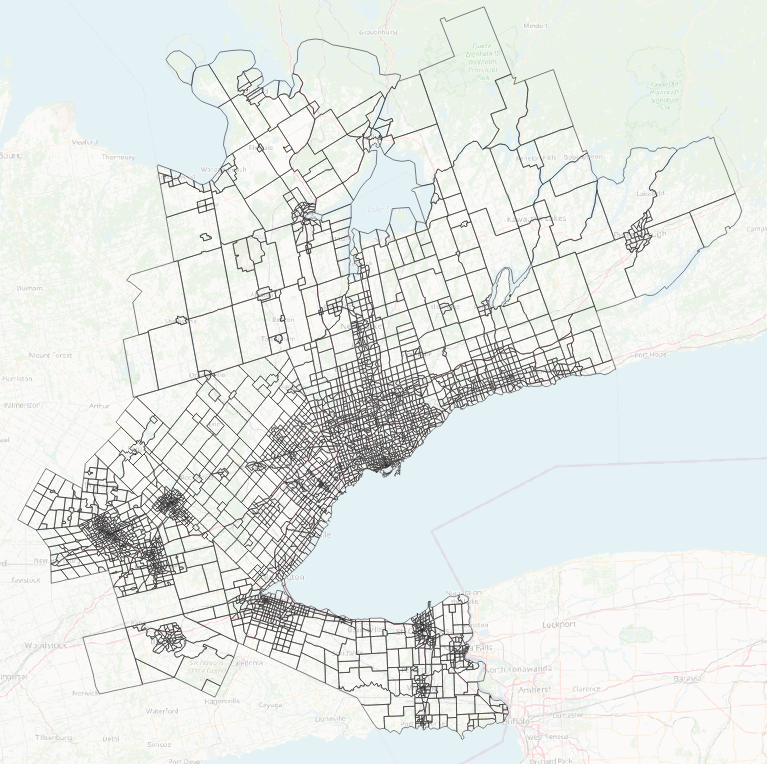
\includegraphics[width=1\linewidth]{images/tts_region.png}
			\end{figure}
			
			
		\end{column}
		
	\end{columns}
	
\end{frame}



\begin{frame}
	
	\textbf{TTS maps} - e.g. car ownership
	
	\begin{figure}
		\centering
		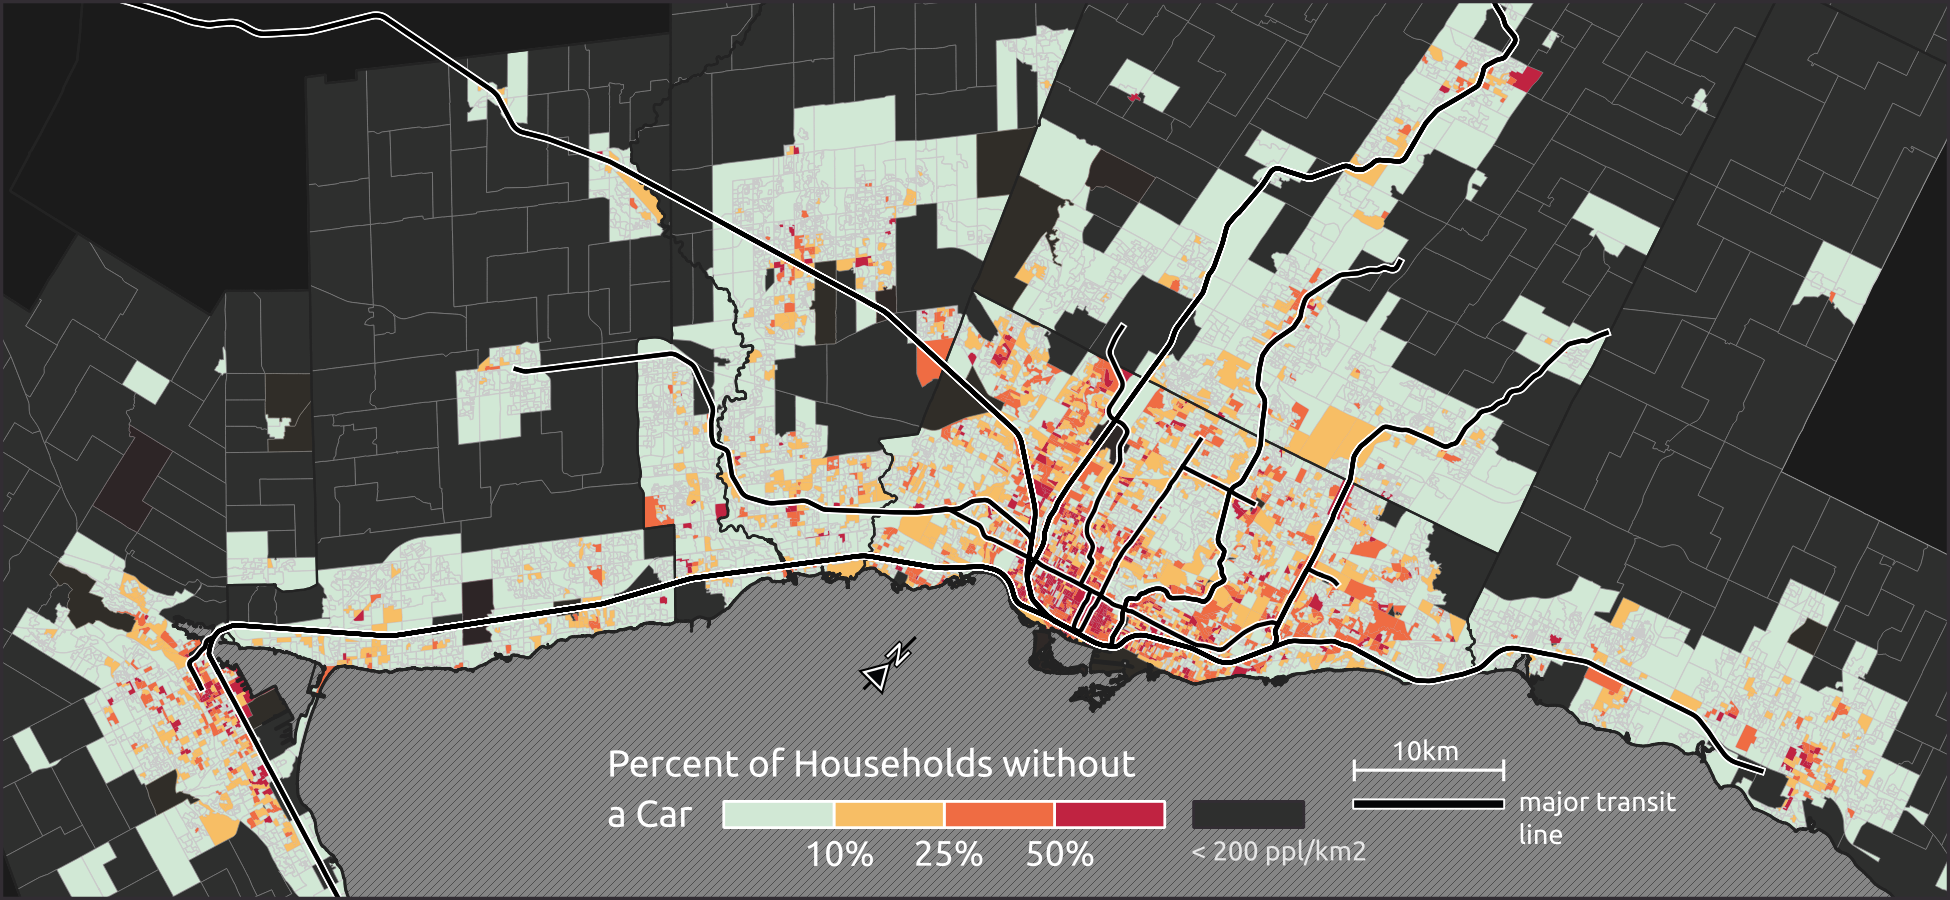
\includegraphics[width=1\linewidth]{images/E_choro_nocar.png}
	\end{figure}

	\tiny Source, me! sorry for the ugly colours
	
\end{frame}



\begin{frame}
	
	\textbf{TTS maps} - e.g. activity participation
	
	\begin{figure}
		\centering
		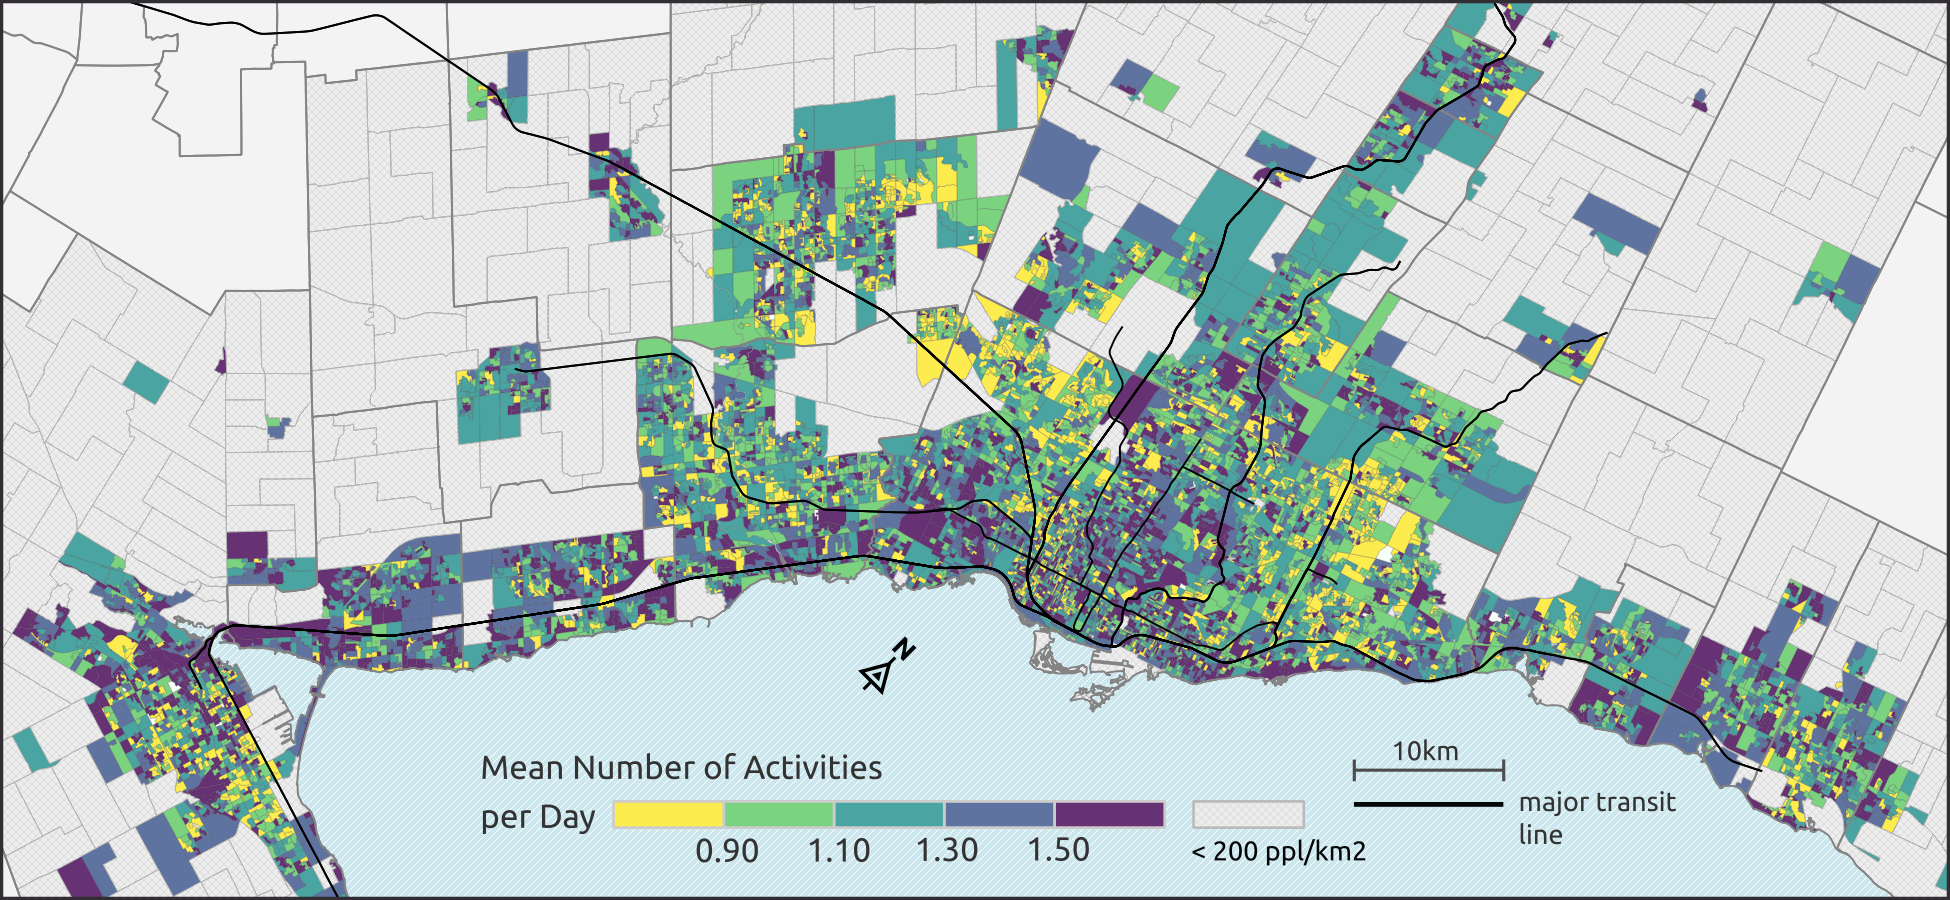
\includegraphics[width=1\linewidth]{images/E_choro_acts.png}
	\end{figure}

	\tiny \url{https://www.sciencedirect.com/science/article/abs/pii/S1361920919308788}
	
\end{frame}



\begin{frame}
	
	\textbf{TTS maps} - e.g. VKT (Vehcile Kilometres Travelled) by workplace
	
	\begin{figure}
		\centering
		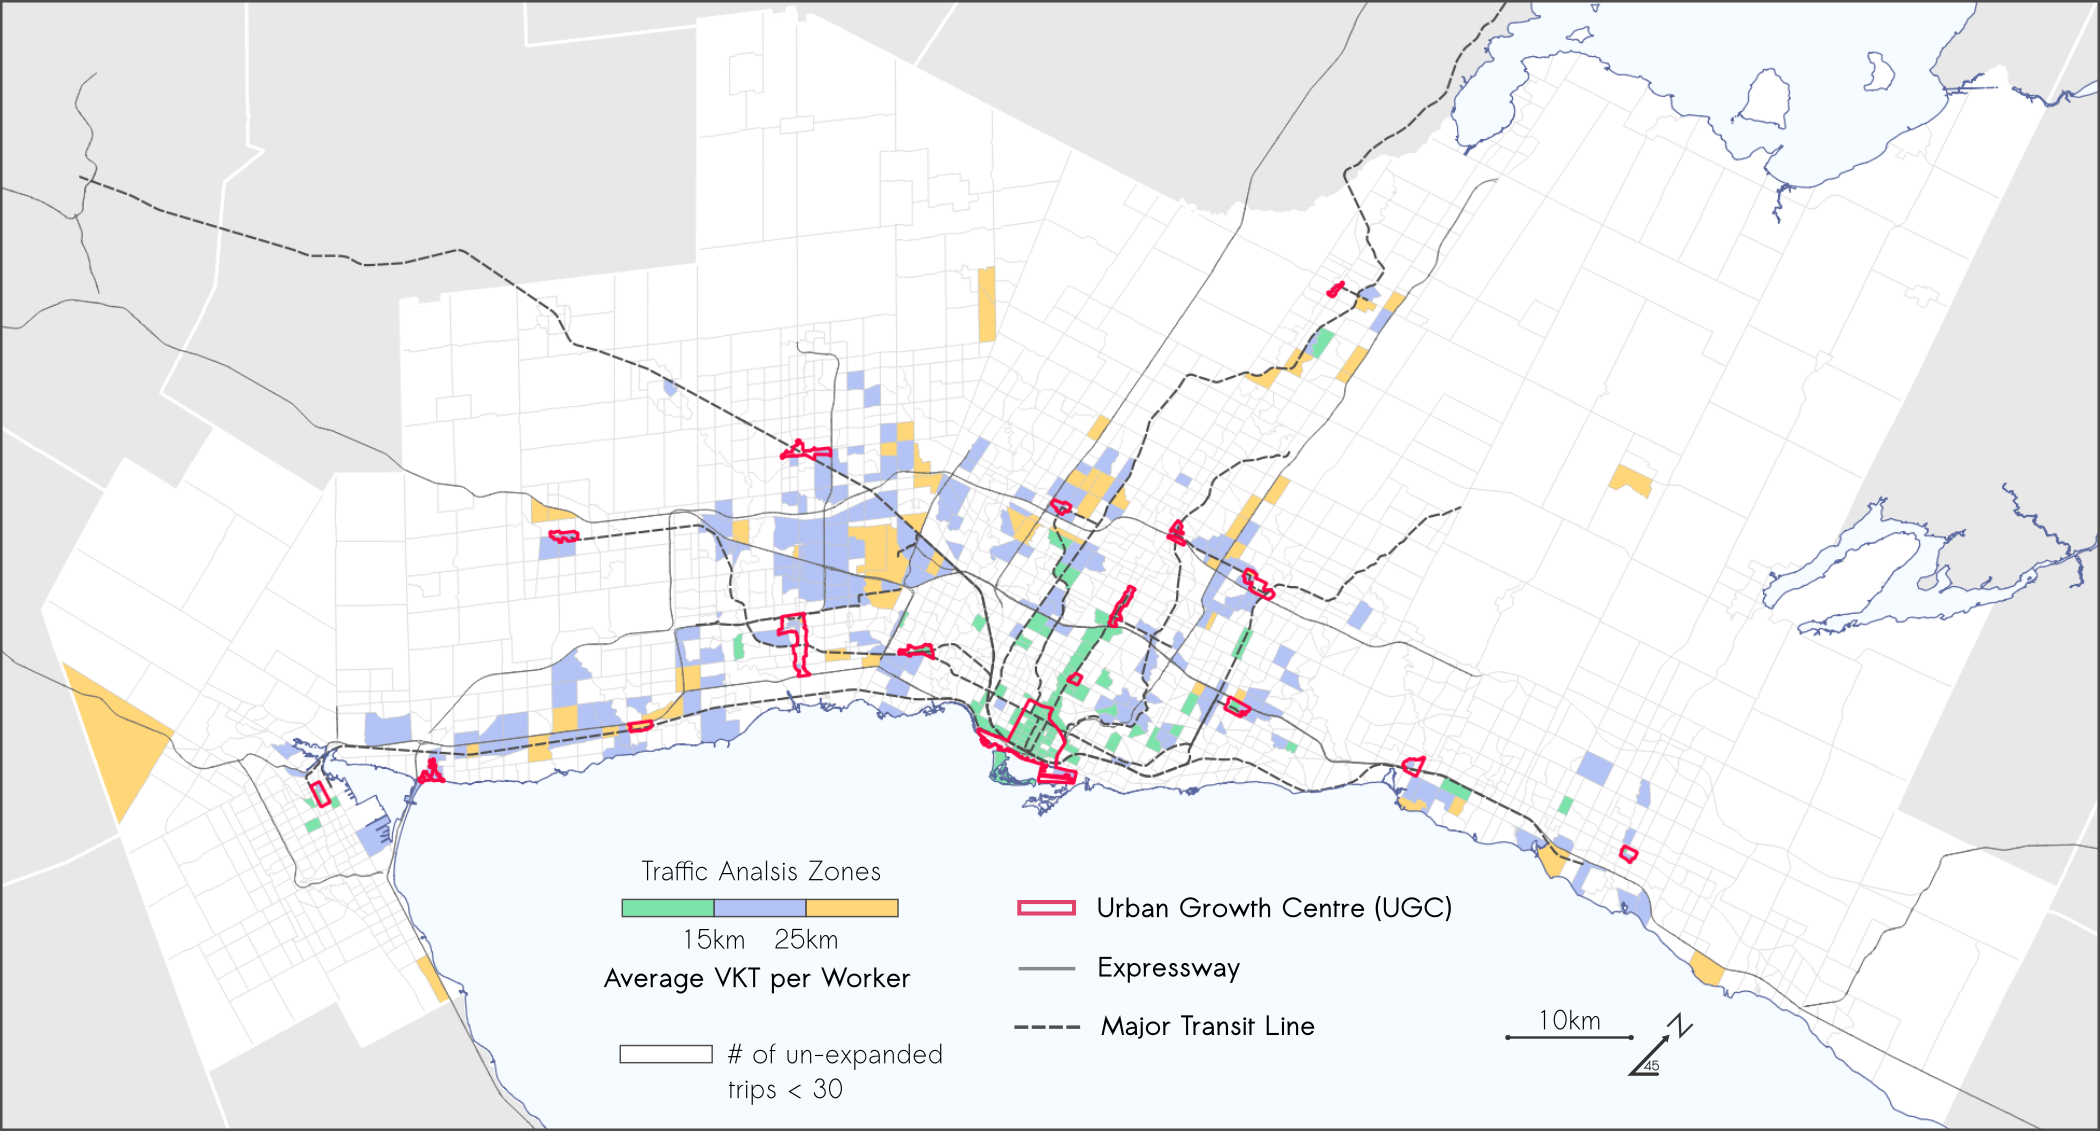
\includegraphics[width=1\linewidth]{images/vkt_map_7.png}
	\end{figure}

	\tiny\url{https://journals.sagepub.com/doi/10.1177/0361198120911053}
	
\end{frame}



\begin{frame}
	
	\textbf{Statistics Canada Survey Data}
	
	\vspace{2mm}
	
	e.g. the long-form Census asks a few questions about commuting
	
	\begin{itemize}
		\item Usual travel mode
		\item Departure time
		\item Travel time
		\item Travel distance
		\item Location of employment
	\end{itemize}
	
\end{frame}


\begin{frame}
	
	\textbf{Summary of 2016 Census}
	
	\begin{figure}
		\centering
		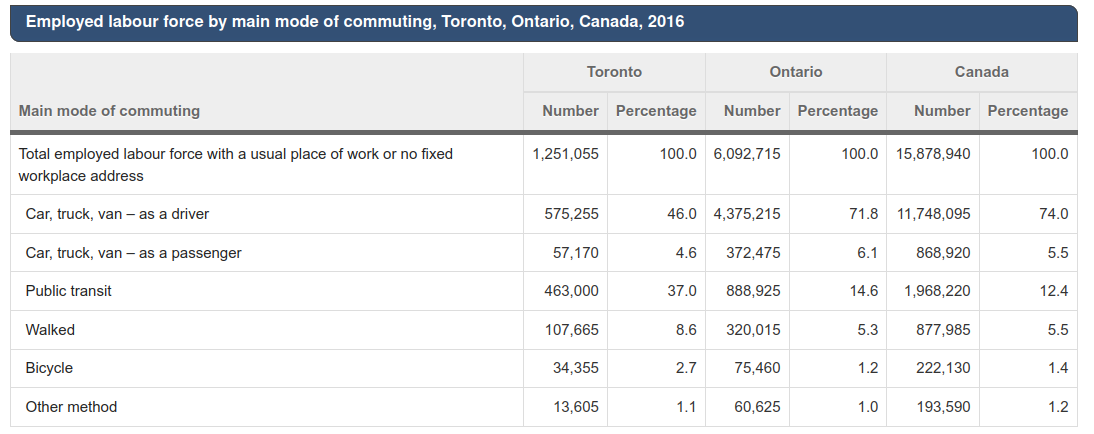
\includegraphics[width=1\linewidth]{images/tor_mode_2016.png}
	\end{figure}
	
	\tiny\url{https://www12.statcan.gc.ca/census-recensement/2016/as-sa/fogs-spg/Facts-cd-eng.cfm?LANG=Eng\&GK=CD\&GC=3520\&TOPIC=12}
	
	
\end{frame}



\begin{frame}
	
	\textbf{Summary of 2016 Census}
	
	\begin{figure}
		\centering
		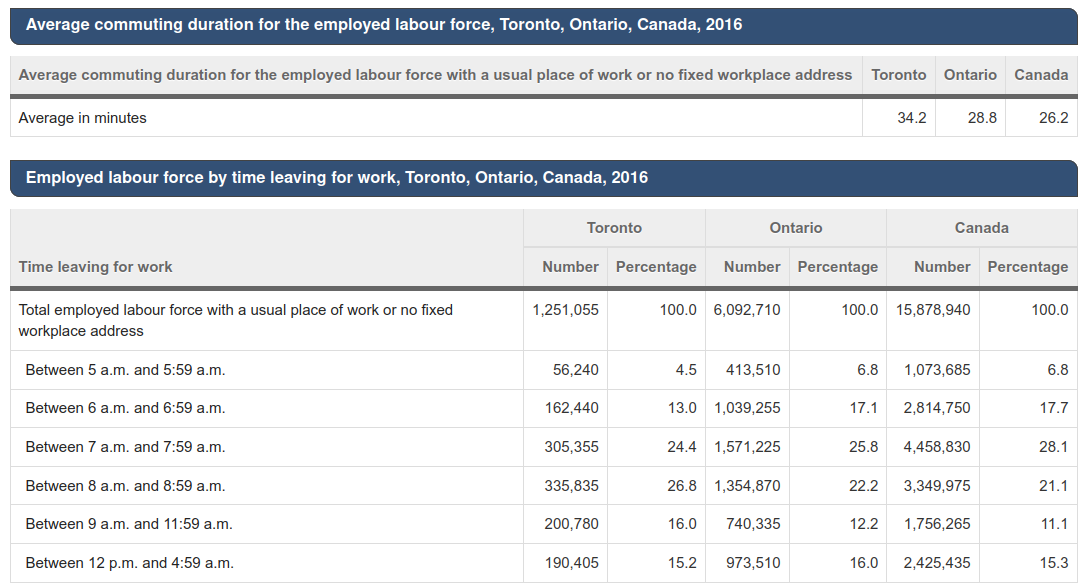
\includegraphics[width=1\linewidth]{images/tor_time_2016.png}
	\end{figure}
	
	\tiny\url{https://www12.statcan.gc.ca/census-recensement/2016/as-sa/fogs-spg/Facts-cd-eng.cfm?LANG=Eng\&GK=CD\&GC=3520\&TOPIC=12}
	
	
\end{frame}



\begin{frame}
	
	\textbf{Summary of 2016 Census}
	
	\begin{figure}
		\centering
		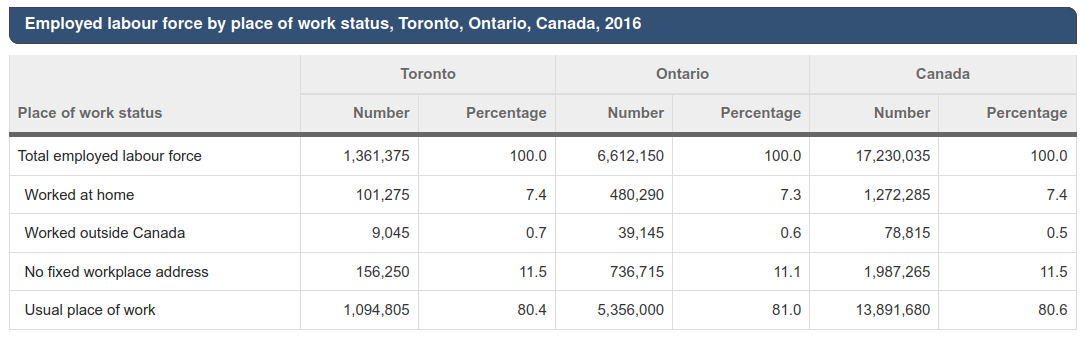
\includegraphics[width=1\linewidth]{images/tor_emp_2016.png}
	\end{figure}
	
	\tiny\url{https://www12.statcan.gc.ca/census-recensement/2016/as-sa/fogs-spg/Facts-cd-eng.cfm?LANG=Eng\&GK=CD\&GC=3520\&TOPIC=12}
	
	
\end{frame}








\begin{frame}
	
	\textbf{Surveys that focus on specific types of questions or sub-populations:}
	\vspace{2mm}
	
	e.g. StudentMoveTO, a travel survey of University students in the GTHA
	
	\begin{figure}
		\centering
		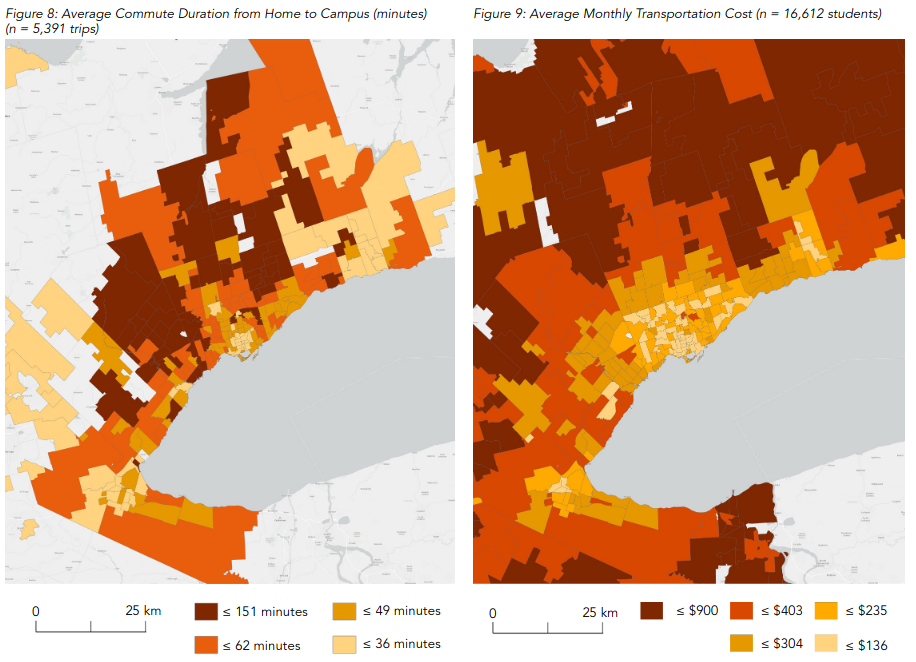
\includegraphics[width=0.7\linewidth]{images/smto_maps.png}
	\end{figure}
	
	\tiny\url{http://www.studentmoveto.ca/resources-2/2019-survey/}
	
\end{frame}






\begin{frame}
	
	\textbf{Travel Surveys}
	
	\vspace{2mm}

Two types of questions

\vspace{2mm}

	\begin{itemize}
		
		\item Revealed preference
		\begin{itemize}
			\item What did you do
			\item \textit{e.g. how did you travel to work today?}
		\end{itemize}
		
		\item Stated preference
		\begin{itemize}
			\item What would you do
			\item \textit{e.g. would you buy an electric vehicle if ... ?}
		\end{itemize}
		
	\end{itemize}
	
\end{frame}




\begin{frame}
	
	e.g. a stated preference survey question, from a survey of transit riders during COVID-19
	\vspace{2mm}
	
	
	\begin{figure}
		\centering
		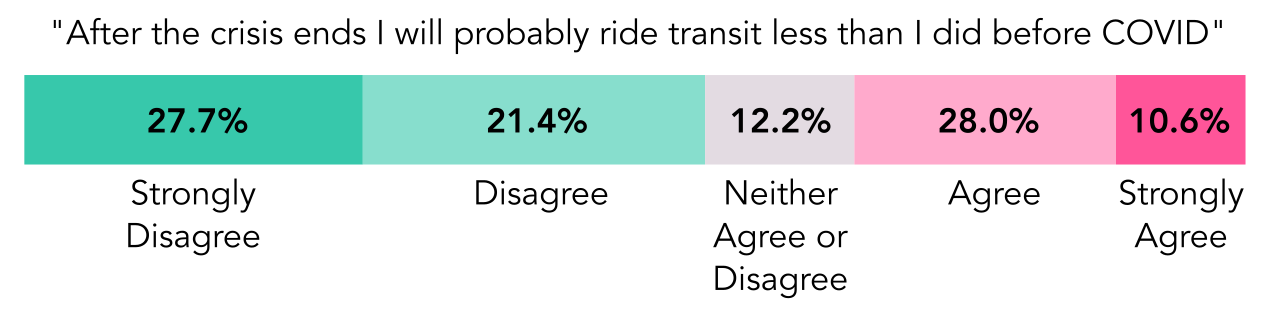
\includegraphics[width=1\linewidth]{images/covid_transit_pref}
	\end{figure}
	
	\tiny$n = 1923$
	
	\vspace{2mm}
	
	\tiny\url{https://tspace.library.utoronto.ca/bitstream/1807/106676/1/ThePublic Transit and COVID-19 Survey Wave2 Results_Final.pdf}
	
\end{frame}








\begin{frame}
	
	\textbf{Travel behaviour data: 2. Observation/Sensor Data}
	
	\begin{itemize}
		\item Instead of asking people, observing how people and vehicles move around a city
		\item Varying levels of technological sophistication
		
		\begin{itemize}
			\item e.g. counting the number of cars in the HOV lane
		\end{itemize}
		
	\end{itemize}
	
	\begin{figure}
		\centering
		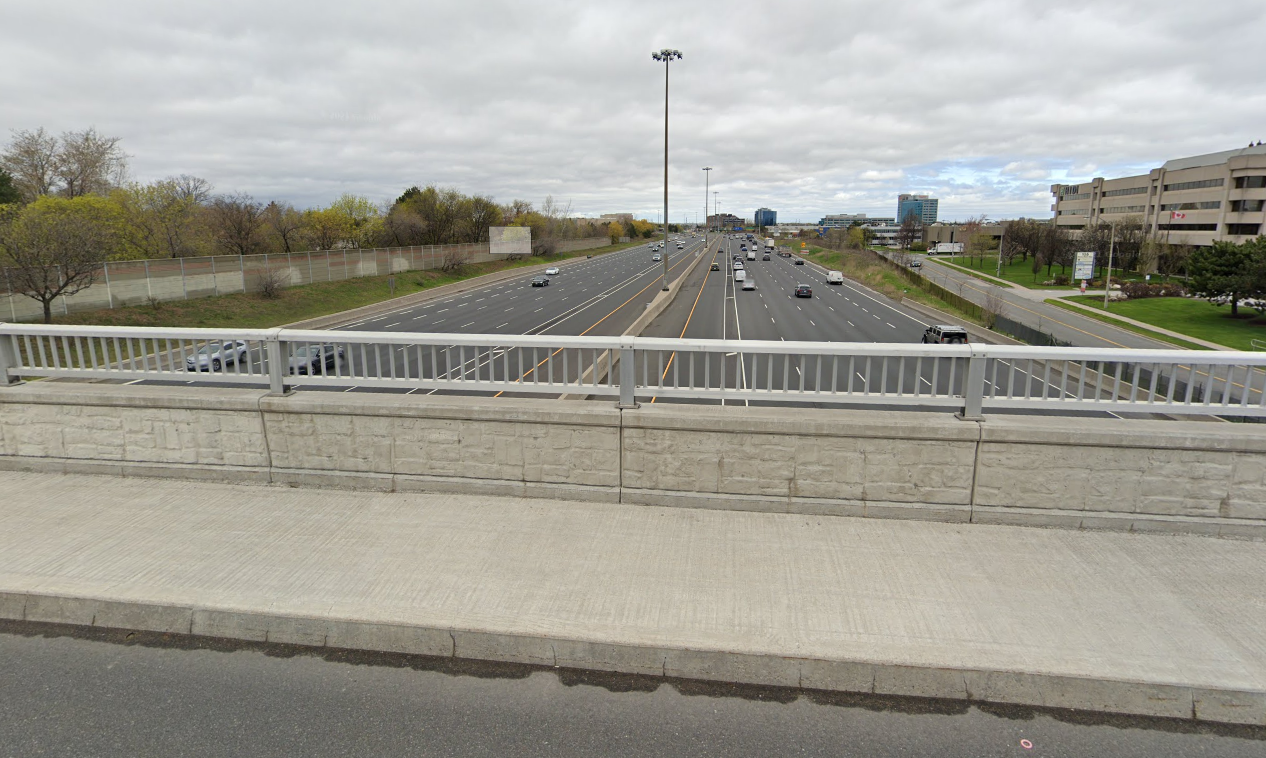
\includegraphics[width=0.7\linewidth]{images/404_bridge.png}
	\end{figure}
	 
\end{frame}









\begin{frame}
	
	Automatic traffic counters
	\vspace{2mm}
	
	e.g. sensors counting cyclists in Copenhagen:
	
	\begin{figure}
		\centering
		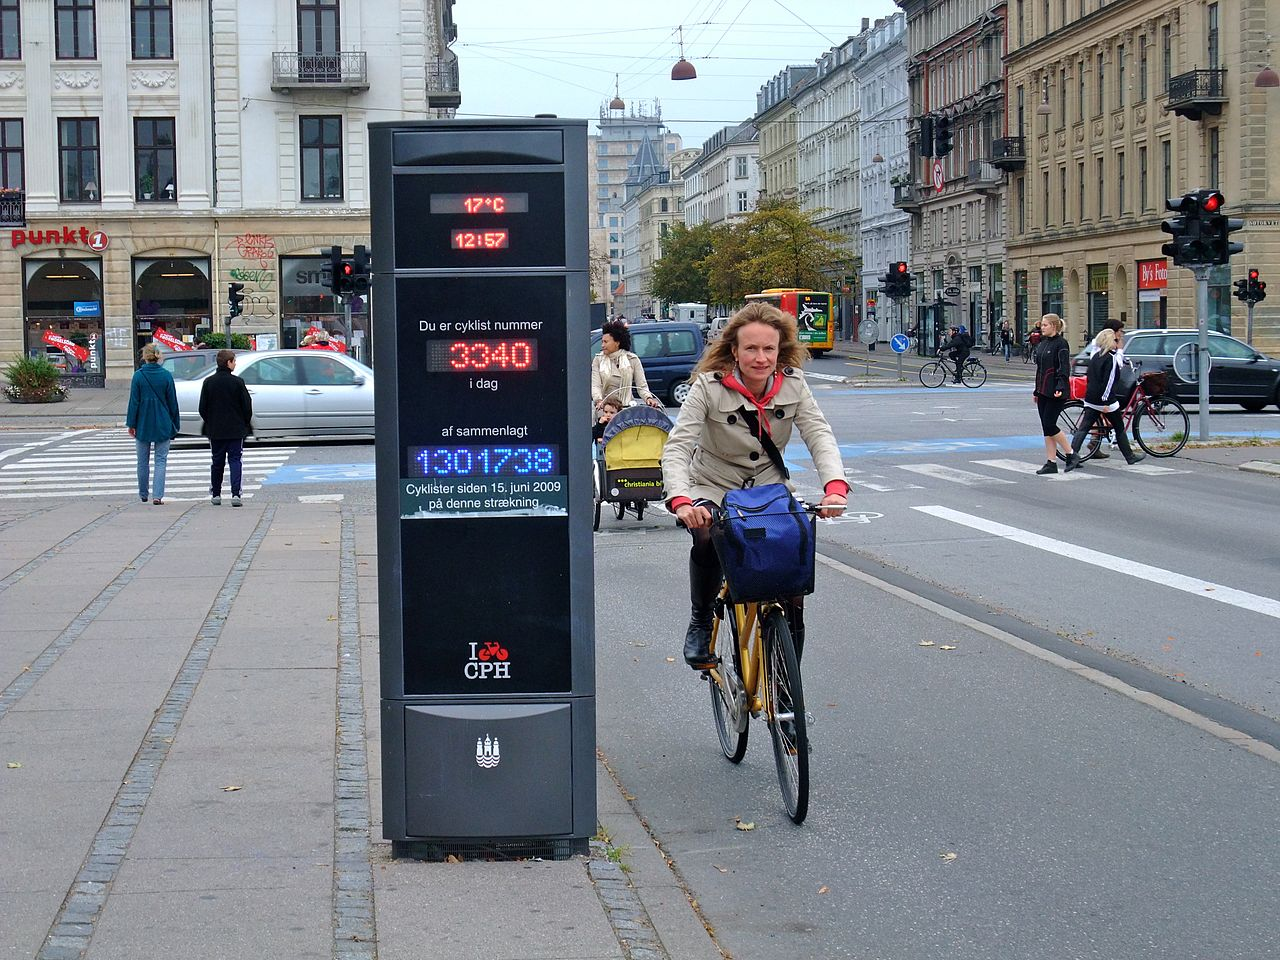
\includegraphics[width=0.7\linewidth]{images/bike_counter_copenhagen}
	\end{figure}
	
	\tiny\url{https://en.wikipedia.org/wiki/Traffic_count}
	
\end{frame}




\begin{frame}
	
	GPS Tracking of vehicles
	
	\begin{figure}
		\centering
		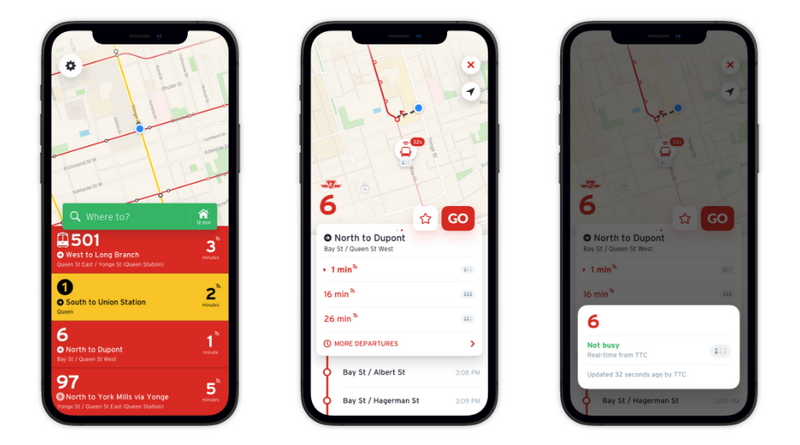
\includegraphics[width=0.7\linewidth]{images/transit_app}
	\end{figure}
	
\end{frame}


\begin{frame}
	
 	Automatic Passenger Counters
	
	\begin{figure}
		\centering
		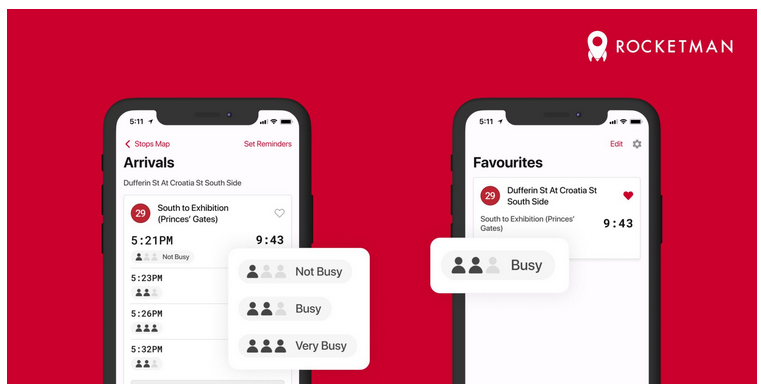
\includegraphics[width=0.7\linewidth]{images/rocketman}
	\end{figure}
	
\end{frame}


% others - e.g. of readings for this week



\begin{frame}
	
	Smartphone GPS Tracking ("passive" data collection on mobility)
	
	\begin{itemize}
		\item e.g. Waze, Google Maps Traffic, etc.
	\end{itemize}
	
	
	
	
	\begin{figure}
		\centering
		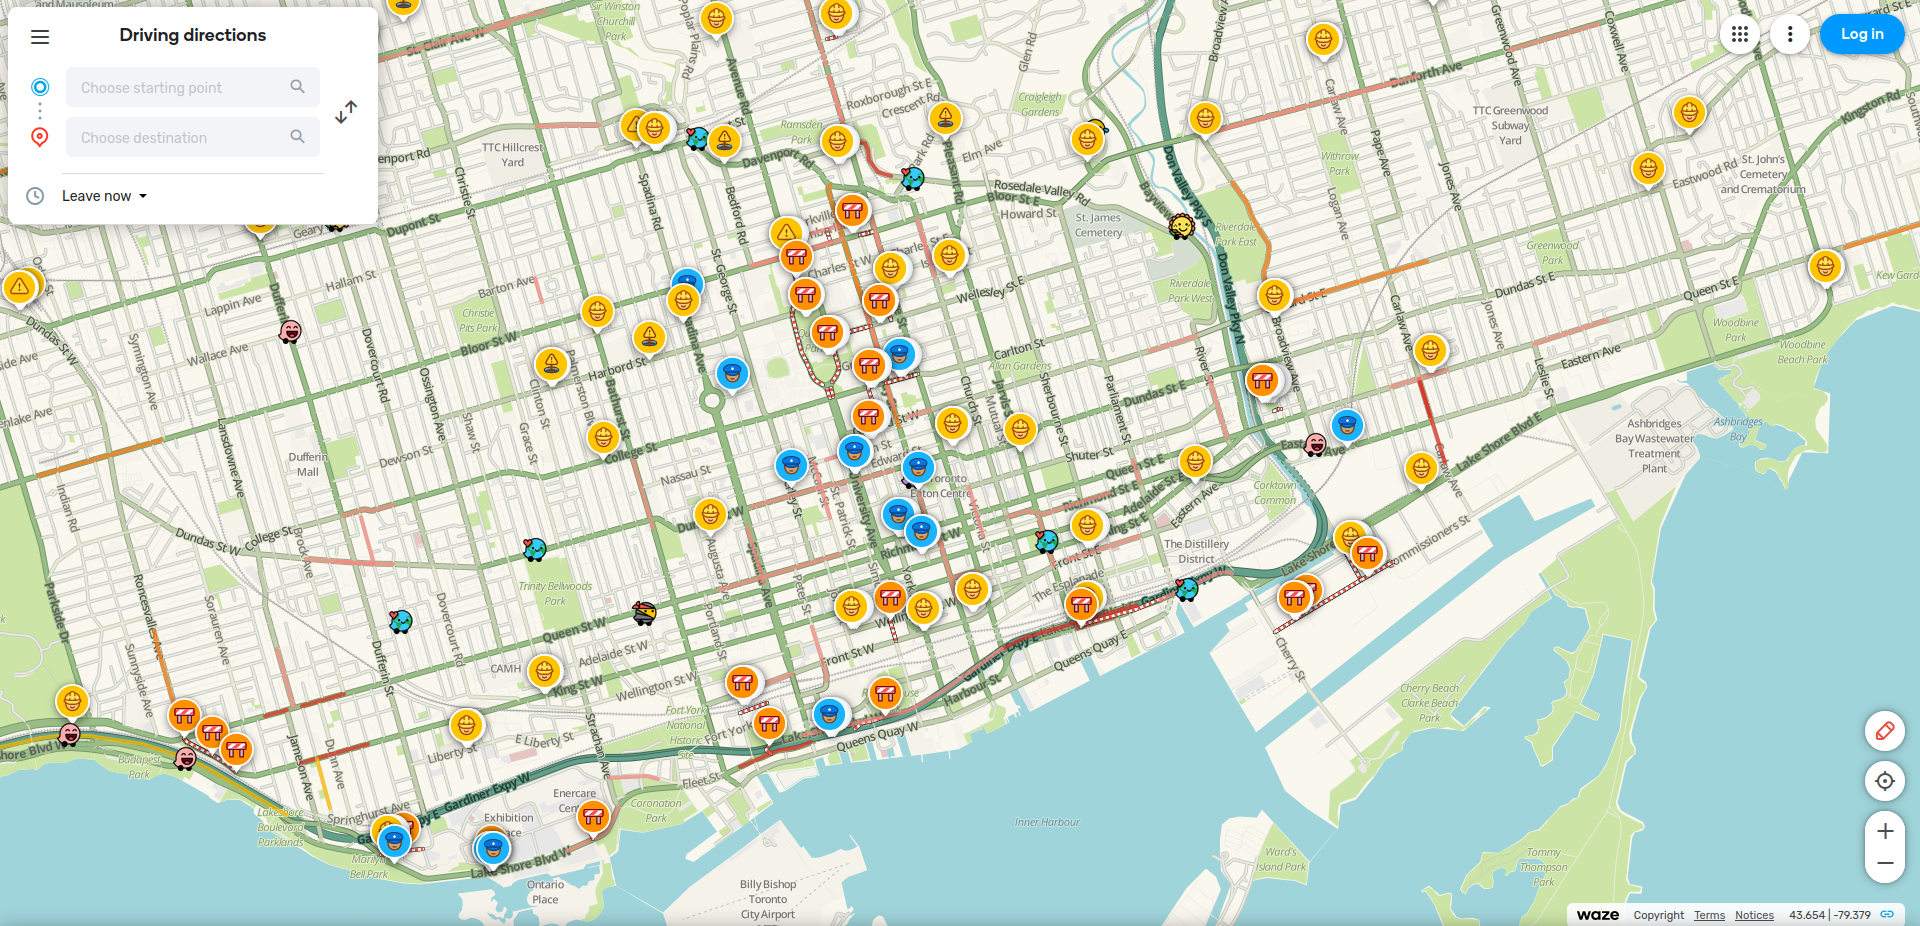
\includegraphics[width=0.8\linewidth]{images/waze.png}
	\end{figure}
	\tiny\url{https://www.waze.com/live-map}
	
\end{frame}



\begin{frame}
	
	Smartphone GPS Tracking ("passive" data collection on mobility)
	
	\begin{itemize}
		\item e.g. NY Times investigation into the smartphone tracking industry
	\end{itemize}
	
	
	\begin{figure}
		\centering
		
\includegraphics[width=0.8\linewidth]{images/nytimes_gps_stockexchange.png}
	\end{figure}
	\tiny\url{https://www.nytimes.com/interactive/2019/12/19/opinion/location-tracking-cell-phone.html}
	
\end{frame}





\begin{frame}
	
	\textbf{After reading week}
	
	\begin{itemize}
		\item In-person class moved to SS2125
		\item Transportation data analysis assignment due March 3
		\item Project proposal due March 10
	\end{itemize}
	
\end{frame}




\end{document}